\section{The finite compiler}\label{sec:compiler}

We prove Lemma~\ref{lem:compiler}. The input is a program index $\eta$
for a partial function $f_\eta:\Sigma^*\rightharpoonup\Sigma^*$ on the
fixed finite alphabet $\Sigma$. We construct a finite monoid presentation
and its partial evaluator. The main issue is to control arbitrary words
in that presentation, including malformed machine configurations.

Encoding a finite machine by contextual equations, and checking the
consequences of using those equations in reverse, are classical ideas
\cite[pp.~3--6]{Post1947}.
Murskii used finite machine presentations to embed finitely generated
recursively presented semigroups in finitely presented semigroups
\cite[Theorem~1.2 and Section~1.5]{Murskii1967}; his construction also
controls malformed initial configurations \cite[Section~2.4]{Murskii1967}.
For the present construction we also need a single evaluator on all
presentation words, normalization paths that never increase grade,
and invariance under equations in arbitrary contexts within the grade
bound. We prove these properties explicitly below.

Fix a deterministic one-tape machine for $f_\eta$, with tape cells indexed
by the nonnegative integers. A left move at cell zero stays there. The
input begins at cell zero and is followed by blanks; a returned string
also begins at zero and ends at its first blank. We use an effective
compilation of the acceptable programming system into this convention.
The resulting finite transition table is part of the compiler's input;
constructing the presentation never runs the program.

\subsection{Cells, paths, and the validator}

A \emph{cell} consists of an immutable base in
$\Sigma\sqcup\{\mathsf C,\mathsf D,\mathsf W\}$ and a finite tag.
Bases in $\Sigma$ are called anchors. The other bases mark two cuts and
a workspace cell. A tag has an anchor-read bit, a workspace-filled bit,
a work symbol from the compiled machine's finite tape alphabet, an
output-reading bit, and an output mark in $\Sigma\sqcup\{\mathrm{none}\}$.
The \emph{clean} tag has every bit unset, work symbol blank, and output
mark none. All these fields may be included on every base; fields not
used there are simply left unchanged. A bare cell base in a rule means
the cell with its entire tag clean.

The presentation has a zero letter $\Omega$ and the arrows of the quiver
in Figure~\ref{fig:compiler-quiver}. There are arrows
$\alpha:O\to L$ and $\omega:R\to O$, head arrows $L\to R$, and two
loop copies $b_L,b_R$ of every tagged cell $b$, at $L,R$, respectively.
There are no vertex-identity generators: the empty word is the global
identity. Add the equations making $\Omega$ absorbing and making every
incompatible pair of arrows equal to $\Omega$.

\begin{figure}[ht]
\centering
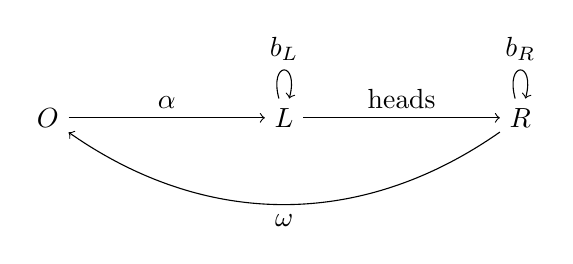
\begin{tikzpicture}[scale=1]
\node (O) at (0,0) {$O$};
\node (L) at (3,0) {$L$};
\node (R) at (6,0) {$R$};
\draw[->] (O) -- node[above] {$\alpha$} (L);
\draw[->] (L) -- node[above] {heads} (R);
\draw[->] (R) to[bend left=35] node[below] {$\omega$} (O);
\draw[->] (L) to[loop above] node[above] {$b_L$} (L);
\draw[->] (R) to[loop above] node[above] {$b_R$} (R);
\end{tikzpicture}
\caption{Nonzero words are paths. Cutting at each interior visit
$\omega\alpha$ to $O$ leaves sectors with at most one head.}
\label{fig:compiler-quiver}
\end{figure}

A nonempty path is cut at every $\omega\alpha$ into \emph{sectors}.
Each contains at most one head, since returning from $R$ to $L$
requires such a cut. A headed sector has optional $\alpha$, left loops,
a head, right loops, and optional $\omega$. Sectors without heads
are allowed. Thus the same notation describes complete computations
and words with missing boundaries.

Assign grade zero to $\Omega$ and workspace cells, grade two to cut cells
with base $\mathsf C$, and grade one to all other generators. Tags do
not affect grade. Extend grade additively to words, writing $\gamma$.
The maximum generator grade is therefore $M=2$. Workspace can be added
without increasing grade, although it increases literal word length.

Use raw and quota heads $\mathsf Q,\mathsf P$, validator heads
$\mathsf I,\mathsf J,\mathsf J',\mathsf N,\mathsf V$, a disjoint set of
machine heads, and a cleanup head $\mathsf Z$.
For an anchor word $x$, the notation $x_L$ or $x_R$ means its sequence
of clean cell copies. A sector is \emph{full raw} if it has the form
\[
\operatorname{raw}(x)=\alpha\mathsf Q x_R\omega,
\qquad x\in\Sigma^*.
\]
The word $x$ is its payload. To combine two such sectors, first impose
\begin{align}
\mathsf Q a_R&=a_L\mathsf Q &&(a\in\Sigma),\label{eq:compiler-slide}\\
\mathsf Q\omega\alpha\mathsf Q&=\mathsf C_L\mathsf P\mathsf D_R,
&\mathsf P\mathsf D_R&=\mathsf W_L\mathsf P\mathsf D_R,
&\mathsf P\mathsf D_R&=\mathsf I\mathsf D_R.
\label{eq:compiler-entry}
\end{align}
In the following validator equations, the arrows specify the forward
direction used to analyze the machine; the defining relations are
equations in both directions:
\begin{align}
\mathsf W_L\mathsf I&\longrightarrow\mathsf I\mathsf W_R,
&\mathsf C_L\mathsf I&\longrightarrow\mathsf J\mathsf C_R,
&a_L\mathsf J&\longrightarrow\mathsf J a_R,\nonumber\\
\alpha\mathsf J&\longrightarrow\alpha\mathsf J',
&\mathsf J'a_R&\longrightarrow a_L\mathsf J',
&\mathsf J'\mathsf C_R&\longrightarrow\mathsf C_L\mathsf N,
\label{eq:compiler-validation}\\
\mathsf N\mathsf W_R&\longrightarrow\mathsf W_L\mathsf N,
&\mathsf N\mathsf D_R&\longrightarrow\mathsf D_L\mathsf V,
&\mathsf V a_R&\longrightarrow a_L\mathsf V,
&\mathsf V\omega&\longrightarrow q_{\rm start}\omega.\nonumber
\end{align}
The anchor rules range over $a\in\Sigma$.

An \emph{entry} has head $\mathsf I$ immediately before clean
$\mathsf D_R$. The validator reaches $q_{\rm start}$ from an entry
only when that entry has the complete form
\begin{equation}\label{eq:compiler-clean-entry}
\alpha x_L\mathsf C_L\mathsf W_L^s\mathsf I\mathsf D_R y_R\omega,
\qquad x,y\in\Sigma^*,\quad s\geq0.
\end{equation}
Indeed the first left sweep checks precisely the clean workspace up to
$\mathsf C$, and the next checks only clean anchors up to $\alpha$.
The rightward sweeps then check these anchors, the first cut, the
workspace, the second cut, and only clean anchors up to $\omega$.
Thus both boundaries and every tag are checked. At the handoff all cells
are on the left of the head.

These relations prepare a raw product for computation. Slide the first
head across $x$, merge the two adjacent heads, insert $s$ workspace
cells, and enter the validator. The simulation and cleanup defined
below will complete the following passage whenever $f_\eta(xy)$ is
defined and has length at most $|xy|$, provided $s$ is sufficiently large:
\begin{equation}\label{eq:compiler-pipeline}
\begin{aligned}
\operatorname{raw}(x)\operatorname{raw}(y)
&\ \rightsquigarrow\ 
\alpha x_L\mathsf C_L\mathsf W_L^s\mathsf I\mathsf D_R y_R\omega\\
&\ \rightsquigarrow\ 
\operatorname{raw}\bigl(f_\eta(xy)\bigr).
\end{aligned}
\end{equation}
The first passage is the preparation just described; the second is
validation, simulation on the workspace, and cleanup. The two anchor
blocks retain the input $xy$ and provide space for its output letters.

Successful computations alone do not control the presented monoid,
because each equation can also be used in reverse. The validator and
simulator will preserve the ordered cell bases and have finitely many
tags and head states. Consequently their transitions on any fixed
sector form a finite graph, even if the simulated program never halts.
We will search its whole weak component---allowing transitions in
either direction---to normalize arbitrary configurations. The component
analysis will distinguish those that contain an entry from those that
do not. Quota insertion is kept outside this finite graph.

\subsection{A finite transition table for the computation}

We specify the remaining machine equations explicitly through finite
scan instructions. This makes the construction uniform in $\eta$ while
avoiding a separate list of rules for each tape symbol.

Every state has one designated reading side. A right-reading state has,
for each tested tagged cell, at most one rule of either form
\begin{equation}\label{eq:compiler-instructions}
q b_R\longrightarrow b'_Lq'
\quad\hbox{or}\quad
q b_R\longrightarrow q'b'_R;
\end{equation}
a left-reading state uses the mirrored forms. These instructions cross
the cell or stay in the same gap, respectively. The cells $b,b'$ always
have the same base. Boundary tests are stationary rules
$\alpha q\to\alpha q'$ or $q\omega\to q'\omega$ on the designated
side. A failed test has no rule. A finite cell predicate expands into
the list of tagged cells satisfying it; complementary cases are
disjoint. Finite registers are incorporated into the state set by a
finite Cartesian product.

Here are the scan instructions used below, together with their complete
expansion convention.
\begin{itemize}
\item To rewind, cross every cell on the left unchanged. At $\alpha$,
  change state without moving and start the specified right-reading
  continuation. If $\alpha$ is absent, the scan gets stuck at the left
  end of the word.
\item To find the first cell satisfying a predicate, test cells on the
  right. At a failure cross unchanged and repeat. At a match use the
  specified stationary update and continuation. At $\omega$, use the
  specified end continuation, or get stuck if failure was prescribed.
\item To go to the right boundary, cross all right cells unchanged and
  use the specified stationary continuation at $\omega$.
\end{itemize}
All invocations are expanded with distinct phase states, apart from
explicit repetitions of a loop. In particular $q_{\rm start}$ is fresh:
its only incoming rule is the validator handoff, and its only outgoing
rule is $q_{\rm start}\omega\to q_{\rm rewind}\omega$, where
$q_{\rm rewind}$ starts the first rewind. No continuation returns to
$q_{\rm start}$ or to a validator state.

The following finite control program supplies all further internal
machine equations.
\begin{enumerate}
\item \emph{Copy the input.} Rewind, and find the first anchor whose read
  bit is unset. Set that bit, carry its base $a$ in finite state, rewind,
  and find the first workspace cell whose filled bit is unset. Write
  $a$ on its work track and set its filled bit. Failure to find that
  workspace cell is stuck. Rewind and repeat the anchor search.

  When the anchor search reaches $\omega$, rewind and check that an
  unfilled workspace cell remains; otherwise get stuck. Rewind once
  more and locate the first workspace cell for simulation. On
  \eqref{eq:compiler-clean-entry} this writes exactly $xy$ in anchor
  order into the initial workspace cells, followed by a blank.

\item \emph{Run the given machine.} The simulated head reads a workspace
  cell on its right. For each machine state and work symbol, expand its
  single transition using \eqref{eq:compiler-instructions}. A stationary
  move writes and stays. A right move writes and crosses the current
  cell, and the next simulation state requires another workspace cell
  on the right. A left move first writes without crossing, then enters
  a left-reading intermediate state. That state crosses an immediately
  left workspace cell unchanged, or stays if the immediately left base
  is $\mathsf C$; any other case is stuck. It then returns to a
  right-reading simulation state. This implements the left-end
  convention. A halt is recognized only at a workspace cell in bounds.

\item \emph{Read the output.} After halt, rewind and find the first
  workspace cell whose output-reading bit is unset. A blank work symbol
  ends the output. For a work symbol $a\in\Sigma$, set that bit, carry
  $a$ in finite state, rewind, and place output mark $a$ on the first
  anchor whose output mark is none. Failure to find such an anchor is
  stuck. Rewind and repeat. An invalid output symbol, or exhaustion of
  the workspace without a blank, is stuck. When output ends, go to
  $\omega$ and enter a fresh state $q_{\rm ok}$, with no outgoing
  internal transition.
\end{enumerate}

Each instruction uses only the finite predicates, finite registers, and
updates just specified. Expanding all cases gives a finite list of
equations computable from the machine table. Each state tests only its
designated side and has disjoint cases. Consequently the internal
forward transition relation has outdegree at most one on \emph{every}
sector, including sectors with missing boundaries and arbitrary tags.
Every transition preserves the number and ordered bases of the cells.

On a passing entry, simulation success computes $f_\eta(xy)$ genuinely.
Conversely, if $f_\eta(xy)$ is defined and has length at most $|xy|$,
then some finite quota $s$ permits success: take more workspace cells
than the input length, the largest tape index visited by the halting
computation, and the output length. The extra cell supplies its blank
delimiter. There are $|xy|$ anchors for the output marks. This includes
empty input: at least one workspace cell is supplied, and a length bound
forces the output to be empty.

Add the exit equation $q_{\rm ok}\omega\to\mathsf Z\omega$ and the
following cleanup equations. An anchor cell $b$ with output mark
$a\in\Sigma$ has
\begin{equation}\label{eq:compiler-cleanup}
b_L\mathsf Z\longrightarrow\mathsf Z a_R.
\end{equation}
For every other tagged cell use $b_L\mathsf Z\to\mathsf Z$, and add
$\alpha\mathsf Z\to\alpha\mathsf Q$. Cleanup is deterministic and
never increases grade, even on dirty data. Applied to a successful
passing entry, it leaves
\begin{equation}\label{eq:compiler-success}
\alpha\mathsf Q f_\eta(xy)_R\omega.
\end{equation}
The leftward sweep places successive output letters on its right in the
correct order. All unused anchors and all nonanchor cells disappear.

\subsection{Finite components on arbitrary sectors}

We now analyze sectors with arbitrary tags and optional boundaries.
For a validator or machine sector, form the graph of internal forward
transitions, excluding entry from $\mathsf P$ and exit to $\mathsf Z$.
We use its entire weak connected component. The ordered bases of its
cells and its boundary flags are fixed. If there are $k$ cells and $h$
internal head states, with at most $c$ tags per cell, there are at most
$(k+1)h c^k$ possible configurations with these data. Its weak component
can therefore be found by a finite search through elementary compiled
steps. This search does not call $f_\eta$ or wait for a computation to
halt. In particular, the quota insertion rule is excluded: finite grade
alone would not bound the number of grade-zero workspace cells.

\begin{lemma}\label{lem:compiler-components}
Every internal weak component has at most one entry and at most one
sector whose head is $q_{\rm ok}$ immediately before its final $\omega$.
If both occur, the forward computation from the entry reaches that
sector and has the clean form and genuine output
described in \eqref{eq:compiler-clean-entry} and
\eqref{eq:compiler-success}.
\end{lemma}
\begin{proof}
An entry has internal indegree zero: the only possible predecessor of an
$\mathsf I$-sector is a left sweep, whose output has clean $\mathsf W$
immediately right of the head, whereas an entry has clean $\mathsf D$.
Every other validator sector has indegree at most one. For head
$\mathsf J$, its possible predecessor types are distinguished by clean
$\mathsf C$ versus an anchor immediately right. For $\mathsf J'$ they
are distinguished by $\alpha$ versus an anchor immediately left; for
$\mathsf N$ by clean $\mathsf C$ versus $\mathsf W$ immediately left;
and for $\mathsf V$ by clean $\mathsf D$ versus an anchor immediately
left. There are no transitions from machine states to validator states.

The validator phases progress in their displayed order, and each sweep
is finite. An entry whose validation fails before handoff therefore
belongs to an isolated finite chain: its vertices have at most one
predecessor and one successor, the entry has no predecessor, and the
failed end has no successor. It shares its component with no other
entry. Every passing entry has
\eqref{eq:compiler-clean-entry}. Its fixed base sequence and boundary
flags determine it uniquely, including its clean tags and the head gap
immediately before the unique $\mathsf D$. Hence there is at most one
entry in any component.

Finally, a finite directed graph with outdegree at most one has a single
eventual cycle or terminal vertex in each weak component. Indeed the
unique forward trajectories of adjacent vertices have the same eventual
object, and this propagates along weak paths. A sector ending in
$q_{\rm ok}\omega$ is terminal. Thus it is the only such sector in its
component, and every forward trajectory there reaches it. If an entry
is present, it therefore passes validation and genuinely succeeds.
\end{proof}

\subsection{The partial evaluator}

The component lemma leaves a choice when both an entry and a successful
terminal occur. Returning to the entry, removing its quota, and undoing
the merge, then sliding the raw heads left, gives
$\operatorname{raw}(x)\operatorname{raw}(y)$;
cleaning up the terminal gives
$\operatorname{raw}(f_\eta(xy))$. We give the entry priority, so that
internal equations have identical preprocessing outputs. The final
combination of consecutive raw sectors will identify the two routes
in \eqref{eq:compiler-pipeline}, using the contextual identity assumed
in Lemma~\ref{lem:compiler} when other raw sectors are adjacent.

This priority also applies to a failed or malformed entry; in that case
quota removal need not produce two full raw sectors. Conversely, a
successful component without an entry need not encode a genuine input
computation. It can use its unique terminal cleanup directly. The
following algorithm includes all these cases.

The algorithm $N_\eta$ preserves the empty word. It sends every word
containing $\Omega$, and every nonpath, to $\Omega$, using the zero
relations. For a nonempty path, first preprocess its sectors as follows.
\begin{enumerate}
\item Leave sectors without heads unchanged. Move $\mathsf Q$ to its
  leftmost reachable gap using \eqref{eq:compiler-slide}, across clean
  anchors only.
\item If $\mathsf P$ has clean $\mathsf D_R$ immediately right, remove
  all immediately preceding clean $\mathsf W_L$ by the quota equation.
  If clean $\mathsf C_L$ is then immediately left, unmerge
  $\mathsf C_L\mathsf P\mathsf D_R$ into
  $\mathsf Q\omega\alpha\mathsf Q$ and normalize the two resulting
  raw heads as above. Otherwise keep the trimmed sector. A
  $\mathsf P$ without immediately right clean $\mathsf D_R$ is kept.
\item Run $\mathsf Z$ cleanup until it is stuck or becomes
  $\mathsf Q$; in the latter case normalize that raw head.
\item For any validator or machine head, find its finite internal weak
  component. If there is an entry, move to it along a weak path, revert
  to $\mathsf P$, and use the preceding rule. If there is no entry but
  there is a sector ending in $q_{\rm ok}\omega$, move there and use
  cleanup. If neither
  exists, use the least sector in the component in shortlex order.
\end{enumerate}
Lemma~\ref{lem:compiler-components} makes the choices in the last rule
unambiguous. The ordering is fixed independently of any grade budget.
All these operations preserve the original outer boundaries; only
unmerge creates an interior $\omega\alpha$ and splits a sector.

Replace each maximal run of $t\geq2$ consecutive full raw sectors,
with payloads $u_1,\ldots,u_t$, by
\begin{equation}\label{eq:compiler-run}
\alpha\mathsf Q f_\eta(u_1\cdots u_t)_R\omega.
\end{equation}
A run of length one is left unchanged, without evaluating $f_\eta$.
This completes the definition of $N_\eta$. Its only calls to that
function are in \eqref{eq:compiler-run}.

Assume now the budget hypothesis of Lemma~\ref{lem:compiler} at $m$.
Every preprocessing operation has a derivation that never raises grade.
Internal component paths preserve every base and hence grade. Raw slides
and entry reversal preserve grade. Quota cells have grade zero. Unmerge
preserves grade because
\[
\gamma(\mathsf C_L\mathsf P\mathsf D_R)=2+1+1
=1+1+1+1=\gamma(\mathsf Q\omega\alpha\mathsf Q).
\]
Cleanup preserves or decreases it. Each argument in
\eqref{eq:compiler-run} has length at most the original total grade,
since every anchor contributes one. Thus all required calls terminate
for an input of grade at most $m$.

The replacement of two full raw sectors is also derivable without
raising grade. Move the first head right across its anchors, merge at
$\mathsf Q\omega\alpha\mathsf Q$, insert a sufficient grade-zero
workspace quota, enter, simulate successfully, and clean up. The result
is the raw word for $f_\eta(u_1u_2)$. Repeating this operation gives
\eqref{eq:compiler-run}, because the budget hypothesis implies
\[
f_\eta\bigl(f_\eta(u_1u_2)u_3\bigr)
=f_\eta(u_1u_2u_3)
\]
and the analogous identities for longer runs. The successive arguments
to $f_\eta$ have length at most $|u_1|+\cdots+|u_t|$, because
$f_\eta$ is length-nonincreasing. Each elementary derivation step
preserves or decreases grade, including the insertion of grade-zero
workspace. Thus every call and every intermediate word remains within
its required budget. This proves termination and the asserted
grade-nonincreasing normalization path.

\subsection{Invariance under equations and contexts}

We verify that one contextual equation step preserves $N_\eta$ when
both endpoints have grade at most $m$. All nonzero equation sides are
nonempty paths with the same initial and terminal vertices. This
includes the deletion $b_L\mathsf Z\to\mathsf Z$. A replacement
therefore preserves whether the whole word is a path. Zero equations
and nonpaths give $\Omega$ on both sides, so it remains to compare paths,
using their sectors in the whole contextualized word.

Raw slides have the same leftmost reachable gap. Quota changes have the
same trimmed sector. Entry from $\mathsf P$ has the same preprocessing
on both sides, since the internal component gives priority to its entry,
even if that entry is malformed and validation fails. Internal
validator or machine equations leave the weak component unchanged.
Cleanup equations give the same result by forward determinism, including
the last step to $\mathsf Q$. A merge is immediately undone by quota
preprocessing before normalizing its two raw heads. This remains true
when the two sectors have incomplete outer boundaries or dirty cells.
In each case the preprocessed sector list is identical, so its subsequent
raw-run replacements agree.

The only remaining equation is
$q_{\rm ok}\omega\to\mathsf Z\omega$. If its internal component has
no entry, both sides use the same unique terminal cleanup. If it has an
entry, Lemma~\ref{lem:compiler-components} says that the entry is
\eqref{eq:compiler-clean-entry} and its computation returns
$f_\eta(xy)$. Entry-priority preprocessing on one side gives two full
raw sectors for $x,y$; cleanup on the other gives a single full raw
sector for $f_\eta(xy)$. With no full raw neighbors, the pair is replaced
by exactly that singleton. Otherwise let $a,b$ be the concatenations of
the neighboring raw words on the left and right. The final runs have
outputs
\[
f_\eta(axyb)
\quad\hbox{and}\quad
f_\eta\bigl(a f_\eta(xy)b\bigr),
\]
which agree by the budget hypothesis. The anchor count $|axyb|$ on the
entry side is at most the original grade, so this use is legitimate.
Passing validation forces both $\alpha$ and $\omega$; an incomplete
sector cannot occur in this exceptional comparison. This proves
equation-step invariance in every context.

If $N_\eta(u)=N_\eta(v)$ and both $xuy,xvy$ have grade at most $m$,
transplant the nonincreasing normalization paths of $u$ and $v$ into
$x(-)y$. Additivity keeps every intermediate word within budget.
Equation-step invariance identifies each input's answer with the answer
of its contextualized normal form. Those two middle strings are
literally equal, proving bounded context compatibility. This argument
does not require sector boundaries to survive the attachment of context.

If the hypotheses hold at every budget, every finite derivation is
covered by some budget. Invariance then implies that equal monoid words
have equal $N_\eta$ answers. The converse follows from each word's
derivation to its answer. Thus $N_\eta$ is an exact word-problem
evaluator. Its definition always leaves each raw singleton
$\alpha\mathsf Q u_R\omega$ literal, distinct from $\Omega$ and from
the empty word; on two such sectors it gives the raw encoding of
$f_\eta(uv)$ whenever the relevant budget hypothesis holds. All parts
of Lemma~\ref{lem:compiler} follow.
